\documentclass{standalone}
  \usepackage{tikz}
  \usetikzlibrary{fit}

  \def\firstcircle{(90:1.75cm) circle (2.5cm)}
  \def\secondcircle{(210:1.75cm) circle (2.5cm)}
  \def\thirdcircle{(330:1.75cm) circle (2.5cm)}

  \begin{document}
    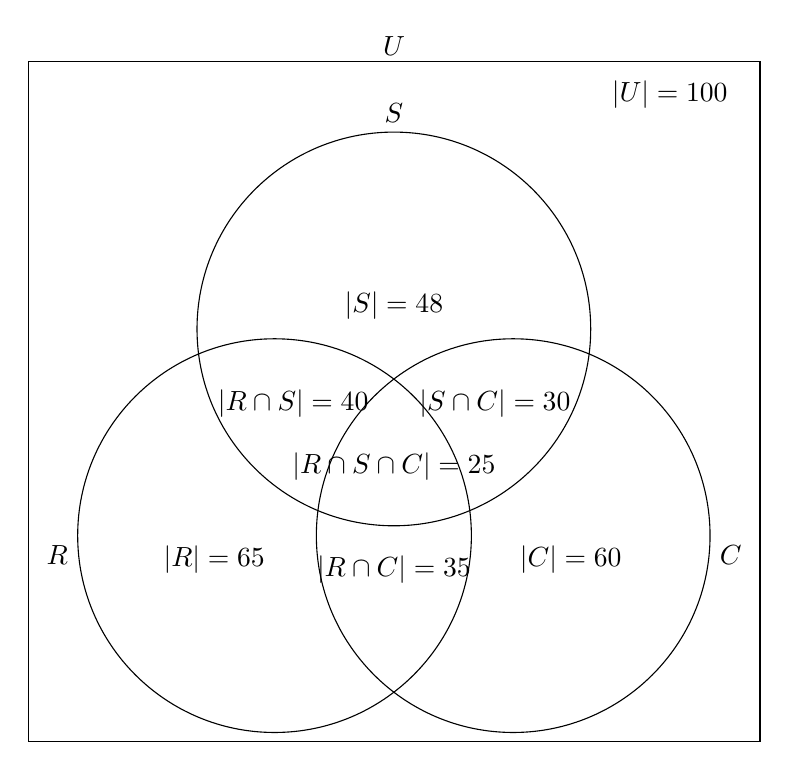
\begin{tikzpicture}
      % \begin{scope}
      %   \clip \secondcircle;
      %   \fill[cyan] \thirdcircle;
      % \end{scope}
    % \begin{scope}
    %   \clip \firstcircle;
    %   \fill[cyan] \thirdcircle;
    % \end{scope}
     

      % Circles
      \begin{scope}[local bounding box = andScope]
        % Swim
        \draw \firstcircle node[text=black, above, yshift=2.5cm] {$S$} node[text=black, above] {$|S|=48$};  

        % Run
        \draw \secondcircle node [text=black, below left, xshift=-2.5cm] {$R$} node [text=black, below left] {$|R|=65$};  

        % Cycle
        \draw \thirdcircle node [text=black,below right, xshift=2.5cm] {$C$} node [text=black, below left, xshift=1.5cm] {$|C|=60$};
       
        % SC
        \draw node[text=black, above right, yshift=0.5cm, xshift=0.2cm] {$|S \cap C|=30$};

        % RS
        \draw node[text=black, above left, yshift=0.5cm, xshift=-0.2cm] {$|R \cap S|=40$};

        % RC
        \draw node[text=black, below, yshift=-1cm] {$|R \cap C|=35$};

        % RSC
        \draw node[text=black] {$|R \cap S \cap C|=25$};

        % U
        \node at (andScope.north) [xshift=3.5cm] {$|U|=100$};
      \end{scope}

      % U
      \node at (andScope.north) [above, yshift=2] {$U$};      

      % Box
      \node[fit=(andScope), draw] {};

    \end{tikzpicture}
  \end{document}